%
% Main document
% ===========================================================================
\documentclass[
    paper=a4,               % paper format
    fontsize=10pt,          % fontsize
    %twoside,               % double-sided
    open=right,             % begin new chapter on right side
    titlepage=false,        % use no standard title page
    parskip=half,           % set paragraph skip to half of a line
]{scrreprt}                 % KOMA-script report
%---------------------------------------------------------------------------
\raggedbottom{}
%\KOMAoptions{cleardoublepage=plain}                                    % Add header and footer on blank pages


% Load Standard Packages:
%---------------------------------------------------------------------------
\usepackage{scrpage2}
\usepackage{pgfgantt}
\usepackage[standard-baselineskips]{cmbright}

\usepackage{scrhack}
\usepackage[ngerman]{babel}                                             % german hyphenation
\usepackage[utf8]{inputenc}                                             % UTF-8 character encoding
\usepackage[T1]{fontenc}                                                % hyphenation of words with ä,ö and ü
\usepackage{textcomp}                                                   % additional symbols
% \usepackage{ae}                                                       % better resolution of Type1-Fonts 
% \usepackage{fancyhdr}                                                 % simple manipulation of header and footer 
\usepackage{etoolbox}                                                   % color manipulation of header and footer
\usepackage{graphicx}                                                   % integration of images
\usepackage{float}                                                      % floating objects
\usepackage[font=footnotesize]{caption}                                 % for captions of figures and tables
\usepackage{booktabs}                                                   % package for nicer tables
\usepackage{tocvsec2}                                                   % provides means of controlling the sectional numbering
\usepackage[square,sort,comma,authoryear]{natbib}                       % provides various citation styles
\usepackage{wrapfig}                                                    % provides floating of text around images
\usepackage{nameref}                                                    % provides printing names of references
\usepackage{paralist}
%---------------------------------------------------------------------------

% Definition of Colors
%---------------------------------------------------------------------------
\RequirePackage{color}                                                  % Color (not xcolor!)
\definecolor{linkblue}{rgb}{0,0,0.8}                                    % Standard
\definecolor{darkblue}{rgb}{0,0.08,0.45}                                % Dark blue
\definecolor{bfhgrey}{rgb}{0.41,0.49,0.57}                              % BFH grey
%\definecolor{linkcolor}{rgb}{0,0,0.8}                                  % Blue for the web- and cd-version!
\definecolor{linkcolor}{rgb}{0,0,0}                                     % Black for the print-version!
\definecolor{codecommentcolor}{rgb}{0, 0.6, 0}                          % Color for code comments
\definecolor{black}{rgb}{0, 0, 0}
\definecolor{maroon}{rgb}{0.5,0,0}
\definecolor{darkgreen}{rgb}{0,0.5,0}
\definecolor{darkblue}{rgb}{0.0,0.0,0.6}
%---------------------------------------------------------------------------

% Load listings package
% which provides source code formatting
%---------------------------------------------------------------------------
\usepackage{xcolor}
\usepackage{listings}                                                   % provides source code formatting
\usepackage{matlab-prettifier}
%---------------------------------------------------------------------------

% Comment package
%---------------------------------------------------------------------------
\usepackage{comment}
%---------------------------------------------------------------------------

% Load Math Packages
%---------------------------------------------------------------------------
\usepackage{amsmath}                                                    % various features to facilitate writing math formulas
\usepackage{amsthm}                                                     % enhanced version of latex's newtheorem
\usepackage{amsfonts}                                                   % set of miscellaneous TeX fonts that augment the standard CM
\usepackage{amssymb}                                                    % mathematical special characters
\usepackage{exscale}                                                    % mathematical size corresponds to textsize
%---------------------------------------------------------------------------

% Package to facilitate placement of boxes at absolute positions
%---------------------------------------------------------------------------
\usepackage[absolute]{textpos}
\setlength{\TPHorizModule}{1mm}
\setlength{\TPVertModule}{1mm}
%---------------------------------------------------------------------------

% Package for annotations
% See http://ctan.mirrorcatalogs.com/macros/latex/contrib/ed/ed.pdf
%---------------------------------------------------------------------------
\usepackage[hide]{ed}
%---------------------------------------------------------------------------

% Hyperref Package (Create links in a pdf)
%---------------------------------------------------------------------------
\usepackage[
    pdftex,ngerman,bookmarks,plainpages=false,pdfpagelabels,
    backref = {false},                                                  % No index backreference
    colorlinks = {true},                                                % Color links in a PDF
    hypertexnames = {true},                                             % no failures "same page(i)"
    bookmarksopen = {true},                                             % opens the bar on the left side
    bookmarksopenlevel = {0},                                           % depth of opened bookmarks
    pdftitle = {Erkennung von aktiven Konturen mittels Matlab},                          % PDF-property
    pdfauthor = {brd3},                                                 % PDF-property
    pdfsubject = {Projektarbeit},                                      % PDF-property
    linkcolor = {linkcolor},                                            % Color of Links
    citecolor = {linkcolor},                                            % Color of Cite-Links
    urlcolor = {linkcolor},                                             % Color of URLs
]{hyperref}
%---------------------------------------------------------------------------

% Cross-reference package
%---------------------------------------------------------------------------
\usepackage{xr}                                                         % provides references to other, external documents
%---------------------------------------------------------------------------
% Set up page dimension
%---------------------------------------------------------------------------
\usepackage{geometry}
\geometry{a4paper,
    left=28mm,
    right=15mm,
    top=30mm,
    headheight=20mm,
    headsep=10mm,
    textheight=242mm,
    footskip=15mm
}
%---------------------------------------------------------------------------

% Makeindex Package
%---------------------------------------------------------------------------
\usepackage{makeidx}                                % To produce index
\makeindex                                      % Index-Initialisation
%---------------------------------------------------------------------------

% Glossary Package
%---------------------------------------------------------------------------
% the glossaries package uses makeindex
% if you use TeXnicCenter do the following steps:
%  - Goto "Ausgabeprofile definieren" (ctrl + F7)
%  - Select the profile "LaTeX => PDF"
%  - Add in register "Nachbearbeitung" a new "Postprozessoren" point named Glossar
%  - Select makeindex.exe in the field "Anwendung" ( ..\MiKTeX x.x\miktex\bin\makeindex.exe )
%  - Add this [ -s "%tm.ist" -t "%tm.glg" -o "%tm.gls" "%tm.glo" ] in the field "Argumente"
%
% for futher informations go to http://ewus.de/tipp-1029.html
%---------------------------------------------------------------------------
\usepackage[nonumberlist]{glossaries}
\makeglossaries{}
\newglossaryentry{aktiver Konturen}
{
    name=Aktive Konturen,
    description={Foos the bar}
}

\newglossaryentry{Segmentationsmethoden}
{
    name=Segmentation,
    description={``Segmentieren beduetet, jedes Pixel einer bestimmten Region zuzuweisen.''~\cite[S. 133]{hudritsch:script:cp}}
}

%---------------------------------------------------------------------------

% Intro:
%---------------------------------------------------------------------------
%\begin{document}                                % Start Document
\settocdepth{section}                                                       % Set depth of toc
\pagenumbering{roman}                                                       
%---------------------------------------------------------------------------

\providecommand{\title}{Erkennung von aktiven Konturen mittels Matlab}
                  % Titel der Arbeit aus Datei titel.tex lesen
% Current version number
\providecommand{\versionnumber}{0.5}

% Date of the current version
\providecommand{\versiondate}{{\today}}
                % Versionsnummer und -datum aus Datei version.tex lesen

% Set up header and footer
%---------------------------------------------------------------------------

\deftripstyle{newlayout}
  [0pt] % no header line
  [0pt] % no footer line
  {}
  {}
  {}
  {\color{bfhgrey} \footnotesize \doctitle, Version \versionnumber, \versiondate}
  {}
  {\color{bfhgrey} \thepage}

\pagestyle{newlayout}
% use "pagestyle" also on chapter starting pages 
\renewcommand{\chapterpagestyle}{newlayout}
\renewcommand{\chaptermark}[1]{\markboth{\thechapter.  #1}{}}
\renewcommand*{\headfont}{\normalfont}
\renewcommand*{\footfont}{\normalfont}
%---------------------------------------------------------------------------

% Randnotizen
\newcommand\mpar[1]{\marginpar{\flushleft\sffamily\small #1}}
\setlength{\marginparwidth}{1.5cm}

\color{black}
\begin{document}

\lstset{
  caption={},
  frame=L,
  basicstyle=\small\normalfont\sffamily,  % the size of the fonts that are used for the code
  stepnumber=1,                           % the step between two line-numbers.
                                          % If it is 1 each line will be numbered
  numbersep=10pt,                         % how far the line-numbers are from the code
  tabsize=2,                              % tab size in blank spaces
  extendedchars=true,                     %
  breaklines=true,                        % sets automatic line breaking
  captionpos=b,                           % sets the caption-position to bottom
  mathescape=true,
  showspaces=false,                       % Leerzeichen anzeigen ?
  showtabs=false,                         % Tabs anzeigen ?
  xleftmargin=17pt,
  framexleftmargin=17pt,
  framexrightmargin=17pt,
  framexbottommargin=5pt,
  framextopmargin=5pt,
  showstringspaces=false                  % Leerzeichen in Strings anzeigen ?
  belowcaptionskip=5em,
  belowskip=3em,
  aboveskip=3em
 }

% Make sure Umlauts are getting displayed correctly.
\lstset{literate=%
    {Ö}{\textcolor{red}{\"O}}1
    {Ä}{{\"A}}1
    {Ü}{{\"U}}1
    {ß}{{\ss}}1
    {ü}{{\"u}}1
    {ä}{{\textcolor{red}{\"a}}}1
    {ö}{{\textcolor{red}{\"o}}}1
    {~}{{\textasciitilde}}1
    {?}{{\textcolor{red}{?}}}1
}

% Title Page and Abstract
%---------------------------------------------------------------------------
\begin{titlepage}

\setlength{\unitlength}{1mm}
\begin{textblock}{20}[0,0](28,12) % chktex-file 36
    
\includegraphics[scale=1.0]{images/BFH_Logo_B.png}
\end{textblock}

\begin{textblock}{154}(28,48)
    \begin{picture}(150,2)
        \put(0,0){\color{bfhgrey}\rule{150mm}{2mm}}
    \end{picture}
\end{textblock}

\begin{textblock}{154}[0,0](26.7,50.5)
    \centering
    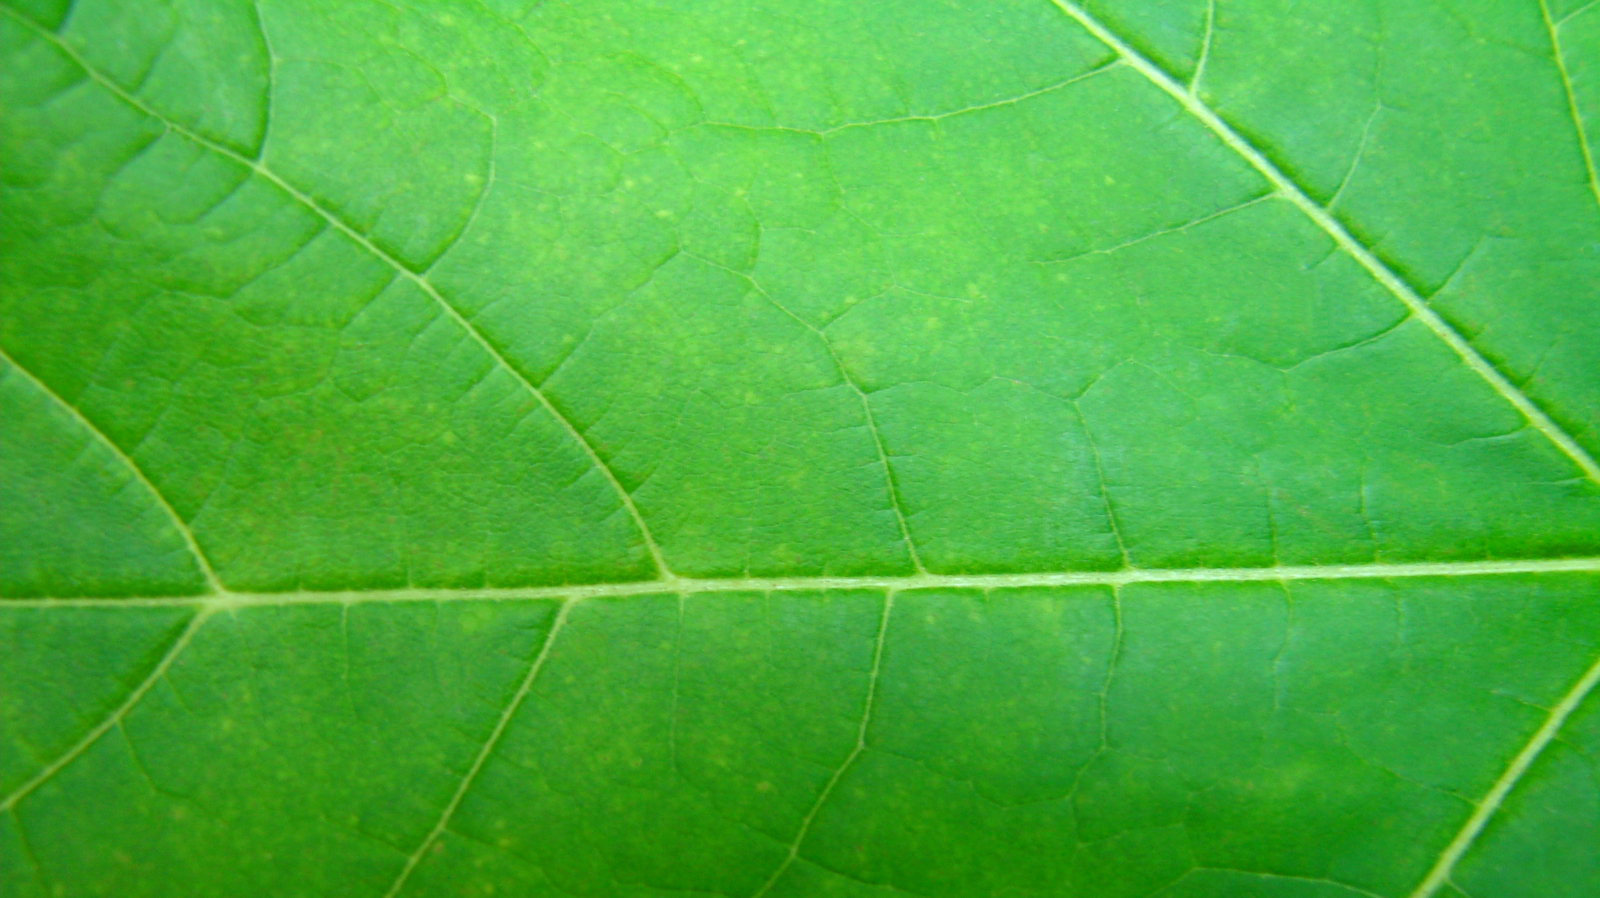
\includegraphics[scale=0.264]{images/title.jpg}\protect\footnotemark{}
\end{textblock}
\footnotetext{Quelle: \url{http://www.freeimages.com/photo/1358335}}

\begin{textblock}{154} (28,135)
    \begin{picture}(150,2)
        \put(0,0){\color{bfhgrey}\rule{150mm}{2mm}}
    \end{picture}
\end{textblock}
\color{black}

\begin{flushleft}

\vspace*{120mm}

\fontsize{26pt}{28pt}\selectfont
Erkennung von aktiven Konturen mittels Matlab
\vspace{3mm}

\fontsize{20pt}{22pt}\selectfont
Projektarbeit
\vspace{3mm}

\fontsize{10pt}{12pt}\selectfont
\textbf{BZG1301: Programmierung mit Matlab/Octave} \\
\vspace{3mm}

\begin{textblock}{150} (28,215)
\fontsize{10pt}{17pt}\selectfont
\begin{tabbing}
xxxxxxxxxxxxxxx\=xxxxxxxxxxxxxxxxxxxxxxxxxxxxxxxxxxxxxxxxxxxxxxx \kill
Autor:        \> Sven Osterwalder\\
Datum:        \> \versiondate\\
Betreuer:     \> Marx Stampfli\\
\end{tabbing}

\end{textblock}
\end{flushleft}

\begin{textblock}{150} (28,280)
\noindent 
\color{bfhgrey}\fontsize{9pt}{10pt}\selectfont
Berner Fachhochschule | Haute école spécialisée bernoise | Bern University of Applied Sciences
\color{black}\selectfont
\end{textblock}


\end{titlepage}

\cleardoublepage{}
\phantomsection{}
\chapter*{}
\label{chap:versionen}

\begin{textblock}{180} (15,150)
\color{black}
\begin{huge}
Versionen
\end{huge}
\vspace{10mm}

\fontsize{10pt}{18pt}\selectfont
\begin{tabbing}
xxxxxxxxxxx\=xxxxxxxxxxxxxxx\=xxxxxxxxxxxxxx\=xxxxxxxxxxxxxxxxxxxxxxxxxxxxxxxxxxxxxxxxxxxxxxx \kill
\textit{Version}	\> \textit{Kalenderwoche}	\> \textit{Status}		\> \textit{Bemerkungen}\\
0.1	\> 9	\> Entwurf		\> Initiale Erstellung des Dokuments\\
0.2	\> 10	\> Entwurf		\> Erstellung Konzept\\
0.3	\> 11	\> Entwurf		\> Verfassen der Einleitung und Grundlagen\\
\end{tabbing}

\end{textblock}

\phantomsection{}
\cleardoubleemptypage{}
\setcounter{page}{1}
\cleardoublepage{}
\phantomsection{}
%\addcontentsline{toc}{chapter}{Versionen}
\cleardoubleemptypage{}
%---------------------------------------------------------------------------

% Summary
%---------------------------------------------------------------------------
\chapter{Zusammenfassung}
\label{chap:summary}
% Die Zusammenfassung wird am zweithäufigsten gelesen. Danach entscheiden viele Leute, ob sie den Bericht weiterlesen oder nicht. In der Zusammenfassung werden Fragestellung und Hypothesen, Methoden, Ergebnisse und Schlussfolgerungen möglichst kurz dargestellt (jeweils etwa zwei bis drei Sätze).

Diese Projektarbeit untersucht, wie gut sich Regionen anhand aktiver Konturen finden lassen. Dies im Gegensatz zu den anderen, bereits in MATLAB verfügbaren Methoden.

Dazu wurde ein Prototyp einer Applikation zur Erkennung aktiver Konturen in Bildern mit Hilfe von MathWorks \gls{MATLAB}~\footnote{\url{http://www.mathworks.com/products/matlab/}} erstellt.

Damit liess sich in einem mit Rauschen behafteten Röntgenbild die definierte Region als zusammenhängend erkennnen.

Ein Vergleich der Lösungen ist unter den gegebenen Umständen jedoch nicht realistisch: Während mittels der MATLAB-internen Methode mehrere Regionen eines Bildes extrahiert werden können, ist dies mit der selbst implementierten Variante zum jetzigen Zeitpunkt nicht möglich.


% Table of contents
%---------------------------------------------------------------------------
% \tableofcontents
% \cleardoublepage{}
%---------------------------------------------------------------------------

% Main part
%---------------------------------------------------------------------------
\pagenumbering{arabic}
\chapter{Einleitung}
\label{chap:intro}

Diese Dissertation ist Teil eines Projektes im Rahmen des Moduls \textit{BZG1301: Programmierung in Matlab/Octave} der Berner Fachhochschule für angewandte Wissenschaft.

Das Ziel dieser Dissertation ist die Umsetzung eines Prototypen einer Applikation mithilfe von MathWorks Matlab~\footnote{\url{http://www.mathworks.com/products/matlab/}} zur Erkennung \gls{aktiver Konturen} in Bildern.

Dabei handelt es sich um eine Möglichkeit ``um in verrauschten Bildern Konturen von Regionen zu bestimmen, die mit anderen \gls{Segmentationsmethoden} nur bedingt als zusammenhängend erkannt werden.''~\cite[S. 144]{hudritsch:script:cp}

Bei dieser Dissertation soll untersucht werden, wie gut sich Regionen anhand aktiver Konturen im Gegensatz zu den herkömmlichen, bereits in Matlab verfügbaren Methoden, finden lassen. Als Daten kommen dabei im Internet gesammelte Bilder zum Einsatz. Es wird erwartet, dass die Regionen, vorallem in verrauschten Bildern, mittels den aktiven Konturen durchgehend als zusammenhängend erkannt werden.

%  Die Einleitung führt die Leserinnen und Leser in die Thematik der Arbeit ein. Sie setzt den Rahmen für die Arbeit, skizziert den aktuellen Wissensstand und geht auf die konkreten Fragestellungen und Ziele der vorliegenden Arbeit ein. Aus der Einleitung muss klar hervorgehen, weshalb die Arbeit gemacht wurde und welche Bedeutung ihr zukommt.
%  
%  \begin{itemize}
%      \item Ziel, worum geht es?
%      \item Eine gute Einleitung motiviert, den ganzen Bericht zu lesen.
%      \item Eine gute Einleitung enthält alle später angesprochenen Themen, aber nur diese!
%      \item Was will ich wissen?
%      \item Was habe ich für Daten? (Wie gesammelt, woher, Weiterarbeit?)
%      \item Welche Modelle brauche ich? (Matlab Toolbox)
%      \item Was erwarte ich von den Resultaten?
%  \end{itemize}

\chapter{Grundlagen}
\label{chap:basics}

% Was muss man als technischen Hintergrund wissen?

Bei aktiven Konturen handelt es sich um eine Art der Segmentierung, also um ein Verfahren der Bildanalyse. Dabei wird ein Bild in interessante und uninteressante Regionen unterteilt, man weist dabei jedes Pixel eines Bildes einer bestimmten Region zu. 

Die aktiven Konturen sind ein Verfahren der modellbasierten Segmentierung, was bedeutet, dass bereits ein gewisses Vorwissen der Grenzen der Segmente vorhanden ist bzw.\ eine Vorstellung davon.

(vgl. \citeauthor*[S. 133 und 144]{hudritsch:script:cp}) % chktex 10 chktex 17 chktex 9

Eine aktive Kontur wird mithilfe von parametrisierten, geschlossenen Kurven beschrieben.

\begin{figure}[H]
    \begin{align}
        r(s) & = (x(s), y(s)), s \in [0,1]
    \end{align}
    \caption{Position einer aktiven Kontur als parametrische Darstellung~\cite{kass88snakes:active}}
\end{figure}

Häufig kommen zur Beschreibung aktiver Konturen B-Spline-Kurven zum Einsatz. Diese haben den Vorteil, dass sie aus mehreren (Kurven-) Segmenten bestehen, welche weiderum aus einigen wenigen Kontrollpunkten bestehen. Die Kontrollpunkte sind zugelich die Koeffizienten der B-Spline-Basisfunktion, dabei ist der Grad der Kurve unabhängig von der Anzahl der Kontrollpunkte. (vgl.~\citeauthor*[S. 79]{fuhrer:script:splines}) % chktex 10 chktex 17 chktex 9

Die Basis einer aktiven Kontur bildet also eine B-Spline-Kurve, deren Kontinuität von Kräften eines Bildes und externen Kräften bestimmt wird. Die internen Kräfte der Kurve ermöglichen eine schrittweise Glättung der Kontur, wohingegen die Kräfte eines Bildes die Kontur zu gewissen Merkmalen, wie z.B. Linen oder Kanten, hinziehen. Die externen Kräfte dienen dazu die Kontur einem gewünschten lokalen Minimum anzunähern. (vgl.~\citeauthor*[S. 323]{kass88snakes:active}) % chktex 10 chktex 17 chktex 9

Aus den genannten Kräften lässt sich, bei parametrischer Darstellung der Position einer aktiven Kontur, folgende Energiefunktion ableiten:

\begin{figure}[H]
    \begin{align}
        E_{snake}^* & = \int_0^1 E_{snake}(v(s))\, \mathrm{d}s\\
         & = \int_0^1 E_{int}(v(s)) + E_{image}(v(s)) + E_{con}(v(s))\, \mathrm{d}s
    \end{align}
    \caption{Energiefunktion einer aktiven Kontur~\cite{kass88snakes:active}}
\end{figure}

Details zu den einzelnen Teilen der Energiefunktion würden den Umfang dieser Arbeit sprengen, daher wird auf eine Beschreibung dieser verzichtet. Details finden sich unter~\citet[S. 247]{hudritsch:script:cp} und unter~\citet[S. 323 bis 328]{kass88snakes:active}.  % chktex 10 chktex 17 chktex 9

\chapter{Konzept}
\label{chap:concept}

% Wie wurde vorgegangen? Gab es Alternativen?

Nachfolgend wird das Vorgehen mittels Zeitplan sowie Meilensteinen beschrieben. Dabei entspricht jeder Meilenstein einem Eintrag im Zeitplan.

\section{Zeitplan}
\label{sec:timetable}

\begin{figure}[H]
    \begin{ganttchart}[
        vgrid,
        x unit=1cm,
        bar/.append style={fill=bfhgrey!50},
    ]{1}{10}
        \gantttitle{2014}{8}
        \gantttitle{2015}{2} \\
        \gantttitlelist{7,...,16}{1} \\ % chktex 11
        \ganttbar{Überlegung Thematik}{1}{1} \\
        \ganttbar{Präsentation Thematik}{2}{2} \\
        \ganttbar{Konzept}{3}{5}
        \ganttbar{}{7}{7}
        \ganttbar{}{9}{9} \\
        \ganttbar{Umsetzung GUI}{4}{5}
        \ganttbar{}{8}{8} \\
        \ganttbar{Implementation}{6}{8} \\
        \ganttbar{Präsentation Ergebnisse}{10}{10}

        \ganttlink{elem0}{elem1}
        \ganttlink{elem1}{elem2}
        \ganttlink{elem2}{elem3}
        \ganttlink{elem3}{elem4}
        \ganttlink{elem4}{elem8}
    \end{ganttchart}
    \caption{Zeitplan; Der Titel stellt Jahreszahlen, der Untertitel Semesterwochen dar}
\end{figure}

\section{Meilensteine}
\label{sec:milestones}

\subsection{Überlegung Thematik}
\label{subsec:topicsearch}
\paragraph{KW 7}
Vor dem eigentlichen Beginn des Projektes wurde mit der Überlegung der Thematik begonnen. Der Entscheid fiel relativ schnell auf die Thematik der aktiven Konturen, da der Autor diese im Schwerpunkt seines Studiums kennengelernt hatte und diese vertiefen wollte. Aktiven Konturen fällt in die Thematik der Bildverarbeitung, wofür Matlab grundsätzlich bestens geeignet ist.

\subsection{Präsentation Thematik}
\label{subsec:topicpres}
\paragraph{KW 8}
Die Thematiken der Teilnehmenden wurde während des Unterrichtes im Fach \textit{BZG1301: Programmierung in Matlab/Octave} vorgestellt, die gewählte Thematik des Autors wurde so vom Donzenten, Herrn Marx Stampfli, angenommen.

\subsection{Konzept}
\label{subsec:concept}
\paragraph{KW 9 bis 11, 13 und 15}
Während der Anfangsphase der Projektarbeit wurde das hier vorliegende Konzept erarbeitet. Dieses wurde dann nach und nach, mit der eigentlichen Umsetzung, erweitert.

\subsection{Umsetzung GUI}
\label{subsec:gui}
\paragraph{KW 10 bis 11, 14}
In einer ersten Phase wurde ein Prototyp der grafischen Benutzeroberfläche zur Anwendung von aktiven Konturen umgesetzt. Dieser war zuerst rudimentär, sprich, ohne Funktion, wurde dann aber schrittweise erweitert.

\subsection{Implementation}
\label{subsec:impl}
\paragraph{KW 12 bis 14}
Bei der eigentlichen Implementation der Lösung wurde der Algorithmus zur Erkennung von aktiven Konturen in Matlab umgesetzt. Zuerst fand eine statische Umsetzung anhand fixer Parameter und eines fixen Bildes statt, schrittweise wurde dann die Implementation mit der grafischen Benutzeroberfläche verknüpft, so dass sich die Parameter mit dieser einstellen und sich das Bild wählen lässt.

\chapter{Material und Methoden}
\label{chap:realisation}

% Was genau wurde gemacht?

In diesem Kapitel wird dargelegt, wie eine bestimmte Untersuchung durchgeführt wurde. Das Material (Pflanzen, Standorte, demographische Daten von Personen etc.), die Beobachtungs- oder Versuchspläne sowie genaue Informationen zu Messungen und zu statistischen Auswertungen werden beschrieben. Neue Methoden werden so beschrieben, dass die Leserinnen und Leser sie nachvollziehen können. Bekannte Methoden werden nur ganz kurz, mit Hinweisen auf die entsprechende Literatur, beschrieben.

Das Kapitel Material und Methoden gilt als unproblematisch, da der Inhalt gut bekannt ist. Es
wird deshalb vorzugsweise als Erstes geschrieben.

\begin{itemize}
    \item Die Leserinnen und Leser lernen die Datenbasis kennen und werden in die Lage versetzt, die Arbeit allenfalls zu wiederholen.
    \item Bei einer Literaturarbeit, die die Ergebnisse anderer Arbeiten zusammenstellt und auswertet, sollte beschrieben werden, wie die verwendete Literatur recherchiert und ausgewertet wurde. Angaben über Suchstrategien und Datenbanken erleichtern das Nachvollziehen der Recherche.
    \item Es muss deutlich werden, wie die Fragen der Einleitung beantwortet werden.
\end{itemize}

\chapter{Vorgehen}
\label{chap:proceeding}
% Dieses Kapitel enthält die gewonnenen Daten und ist deshalb in wissenschaftlicher Hinsicht besonders wichtig. Es dürfen nur Ergebnisse, die für die Fragestellung relevant sind, aufgeführt werden. Dazu können aber auch Negativergebnisse gehören. Die Fragen der Einleitung müssen mit den vorgestellten Ergebnissen zu beantworten sein.
% 
% Die Ergebnisse sollten mit Hilfe von Abbildungen und Tabellen möglichst übersichtlich dargestellt werden. Der Text sollte möglichst kurz gehalten werden und nicht die Informationen der Abbildungen und Tabellen wiederholen. Emotionen wie z.B. Erstaunen oder Entsetzen sollten vermieden werden. In den statistischen Auswertungen müssen neben Mittelwerten auch Streuungsmasse und Stichprobengrössen angegeben werden.
% 
% Es muss immer klar sein, ob es sich um eigene oder fremde Ergebnisse (z.B. aus Literaturrecherchen) handelt. Bei fremden Ergebnissen muss im Text auf die Herkunft verwiesen werden (siehe 2.8). Wörtliche Zitate sollten vermieden werden.

%  \begin{compactenum}[a)] % chktex 9 chktex 10 chktex 17
%      \item Auszug aus einer zoologischen Untersuchung zur Diversität von Arthropoden in voralpinen Flachmooren:
%          „In den untersuchten Gebieten konnten 63 Tagfalterarten aus 6 Familien nachgewiesen werden (Anhang IV). 16 Arten (25\%) gelten als typische Moorindikatoren und 23 Arten (37\%) erscheinen auf der Roten Liste der gefährdeten Tagfalter der Schweiz (Duelli 1994). Die Individuenzahl der Arthropoden nahm mit zunehmender Höhe ab (p < 0.05). Während in der tiefen Höhenstufe durchschnittlich 249 Tiere pro Gebiet gefangen wurden, waren es in der mittleren Höhenstufe 236 und in der höchsten nur noch 191 Individuen.“
%      \item Auszug aus einer sozialwissenschaftlichen Untersuchung über Engagement und Mobilität:
%          „Die Gesamtmobilität der Befragten liegt bei 12'600 km (Bezugsjahr 1994). Sie hat im erfragten Zeitraum um 12\% zugenommen (von 11'300 km auf 12'600 km). Der grösste Teil dieses Anstiegs geht auf die Ferienmobilität zurück, die im Schnitt von 6'400 km auf 7'300 km zugenommen hat. Die genannten Mobilitätswerte liegen deutlich unter dem Schweizer Durchschnitt.“
%  \end{compactenum} % chktex 17

Ziel dieser Projektarbeit war es, ein eigenes Programm zur Erkennung von Regionen mittels aktiver Konturen zu entwickeln und ursprünglich mit anderen, in MATLAB verfügbaren Methoden zu vergleichen.

\section{Ausgangslage}
\label{sec:proceeding:basics}
Als Grundlage für die methodischen Vergleiche wurde eine angepasste Version des Bildes~\footnote{\url{http://upload.wikimedia.org/wikipedia/commons/3/3d/Patella_bipartita.jpg}} verwendet, wie in Abbildung~\ref{fig:source_img} ersichtlich.

\begin{figure}[h!]
    \centering
    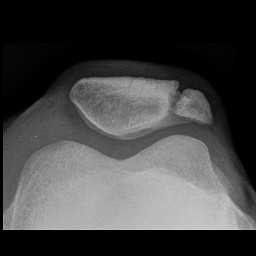
\includegraphics[scale=0.5]{images/patella_bipartita.jpg}
    \caption{Quellbild der Versuche\protect\footnotemark{}}
\label{fig:source_img}
\end{figure}
\footnotetext{Angepasste Version von \url{http://upload.wikimedia.org/wikipedia/commons/3/3d/Patella_bipartita.jpg}}

Die zu vergleichenden Methoden sollen die Fraktur der Kniescheibe, wie in~\autoref{fig:target_img} ersichtlich, als zusammenhängende Region erkennen.

\begin{figure}[h!]
    \centering
    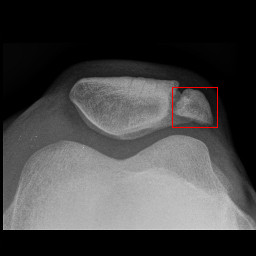
\includegraphics[scale=0.5]{images/patella_bipartita_target.jpg}
    \caption{Quellbild der Versuche mit eingezeichneter Zielregion\protect\footnotemark{}}
\label{fig:target_img}
\end{figure}
\footnotetext{Angepasste Version von \url{http://upload.wikimedia.org/wikipedia/commons/3/3d/Patella_bipartita.jpg}}

\newpage

\section{Angewendete Methoden}
\label{sec:proceeding:methods}
\begin{itemize}
    \item Entwicklung einer Applikation zur Erkennung von Regionen mittels aktiven Konturen
    \item MATLAB-interne Methode \textit{activecontour} als Vergleich
\end{itemize}

Zur Erkennung der Region mittels den in MATLAB vorhandenen Methoden wurde die \textit{activecontour}-Methode (siehe~\footnote{\url{http://www.mathworks.com/help/images/ref/activecontour.html}}) der ``Image Processing Toolbox'' (siehe~\footnote{\url{http://www.mathworks.com/products/image/}}) verwendet. Als Eingabe-Parameter wurden dazu die unter~\ref{fig:matlab_mask} abgebildete Maske, 300 Iterationen sowie das kantenbasierte Verfahren gewählt.

\begin{figure}[h!]
    \centering
    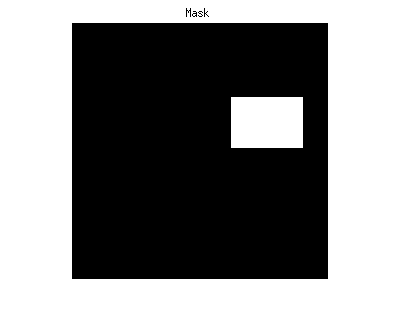
\includegraphics[scale=0.5]{images/matlab_mask.png}
    \caption{Maske zur Erkennung der gewünschten Region\protect\footnotemark[6]{}}
\label{fig:matlab_mask}
\end{figure}
\footnotetext[6]{Eigene Darstellung mittels MATLAB}

Die Untersuchung mittels anderer Methoden erwies sich als zu aufwändig. Bewusst wurde darauf verzichtet.

Bei der eigenen Implementation wurden zur Erkennung der Region die in Abbildung~\ref{fig:ownimpl_contour} ersichtlichen Punkte gewählt. Als Eingabe-Parameter wurden für die Elastizität ($\alpha$) \textit{0.54}, für die Kurvatur ($\beta$) \textit{0.1} und für die Energie des Bildes ($\gamma$) \textit{0.9} genommen. Diese Werte basieren einerseits auf~\cite[Seite 148]{hudritsch:script:cp}, andererseits auf eigenen Versuchen.

\begin{figure}[h!]
    \centering
    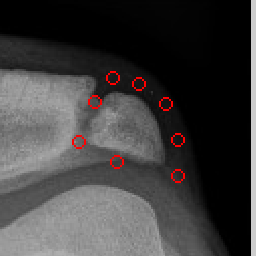
\includegraphics[scale=0.5]{images/ownimpl_contour.png}
    \caption{Definierte Punkte zur Bildung der aktiven Kontur\protect\footnotemark[6]{}}
\label{fig:ownimpl_contour}
\end{figure}

Als Eingabe zur Bildung der aktiven Kontur wurde das Binärbild mit den erkannten Kanten des Bildes, wie unter~\ref{fig:ownimpl_edges} ersichtlich, gewählt. Die Bildung der aktiven Kontur wurde mit 1000 Iterationen durchgeführt.

\begin{figure}[H]
    \centering
    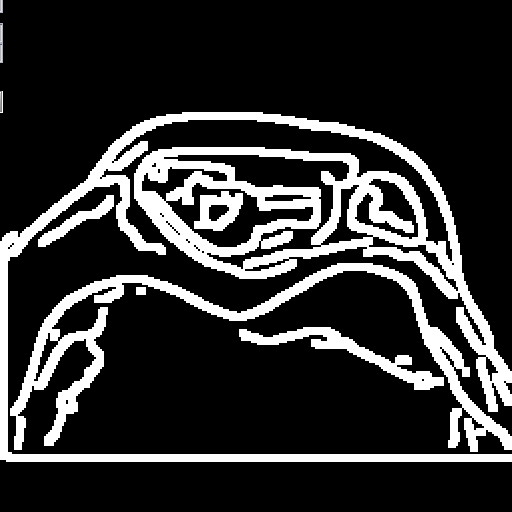
\includegraphics[scale=0.25]{images/ownimpl_edges.png}
    \caption{Binärbild mit den erkannten Kanten des Bildes\protect\footnotemark[6]{}}
\label{fig:ownimpl_edges}
\end{figure}

\chapter{Ergebnisse}
\label{chap:results}

% Dieses Kapitel enthält die gewonnenen Daten und ist deshalb in wissenschaftlicher Hinsicht besonders wichtig. Es dürfen nur Ergebnisse, die für die Fragestellung relevant sind, aufgeführt werden. Dazu können aber auch Negativergebnisse gehören. Die Fragen der Einleitung müssen mit den vorgestellten Ergebnissen zu beantworten sein.
% 
% Die Ergebnisse sollten mit Hilfe von Abbildungen und Tabellen möglichst übersichtlich dargestellt werden. Der Text sollte möglichst kurz gehalten werden und nicht die Informationen der Abbildungen und Tabellen wiederholen. Emotionen wie z.B. Erstaunen oder Entsetzen sollten vermieden werden. In den statistischen Auswertungen müssen neben Mittelwerten auch Streuungsmasse und Stichprobengrössen angegeben werden.
% 
% Es muss immer klar sein, ob es sich um eigene oder fremde Ergebnisse (z.B. aus Literaturrecherchen) handelt. Bei fremden Ergebnissen muss im Text auf die Herkunft verwiesen werden (siehe 2.8). Wörtliche Zitate sollten vermieden werden.

%  \begin{compactenum}[a)] % chktex 9 chktex 10 chktex 17
%      \item Auszug aus einer zoologischen Untersuchung zur Diversität von Arthropoden in voralpinen Flachmooren:
%          „In den untersuchten Gebieten konnten 63 Tagfalterarten aus 6 Familien nachgewiesen werden (Anhang IV). 16 Arten (25\%) gelten als typische Moorindikatoren und 23 Arten (37\%) erscheinen auf der Roten Liste der gefährdeten Tagfalter der Schweiz (Duelli 1994). Die Individuenzahl der Arthropoden nahm mit zunehmender Höhe ab (p < 0.05). Während in der tiefen Höhenstufe durchschnittlich 249 Tiere pro Gebiet gefangen wurden, waren es in der mittleren Höhenstufe 236 und in der höchsten nur noch 191 Individuen.“
%      \item Auszug aus einer sozialwissenschaftlichen Untersuchung über Engagement und Mobilität:
%          „Die Gesamtmobilität der Befragten liegt bei 12'600 km (Bezugsjahr 1994). Sie hat im erfragten Zeitraum um 12\% zugenommen (von 11'300 km auf 12'600 km). Der grösste Teil dieses Anstiegs geht auf die Ferienmobilität zurück, die im Schnitt von 6'400 km auf 7'300 km zugenommen hat. Die genannten Mobilitätswerte liegen deutlich unter dem Schweizer Durchschnitt.“
%  \end{compactenum} % chktex 17

\section{MATLAB-interne Methode \textit{activecontour}}
\label{sec:results:matlab}
Mittels der MATLAB-internen Methode wurde die Fraktur als zusammenhängende Region erkannt und könnte somit problemlos extrahiert werden. Die Erkennung dauert im Schnitt rund 4.3 Sekunden. Das Resultat ist in Abbildung~\ref{fig:matlab_result} ersichtlich.

\begin{figure}[h!]
    \centering
    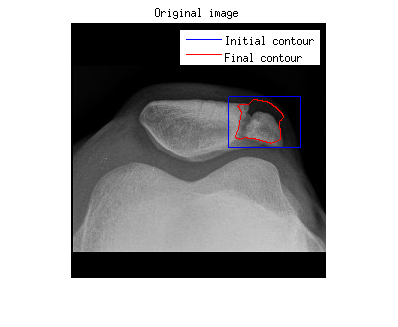
\includegraphics[scale=0.6]{images/matlab_result.png}
    \caption{Resultat der Erkennung der gewünschten Region mittels der MATLAB-internen Methode \textit{activecontour}\protect\footnotemark[1]{}}
\label{fig:matlab_result}
\end{figure}
\footnotetext[1]{Eigene Darstellung mittels MATLAB}

\section{Eigene Implementation}
\label{sec:results:own}
Auch mit dieser Methode wurde die Fraktur als zusammenhängende Region erkannt und könnte somit problemlos extrahiert werden. Die Erkennung dauert im Schnitt rund 3.5 Sekunden. Das Resultat ist in~\autoref{fig:ownimpl_result} abgebildet.

\begin{figure}[h!]
    \centering
    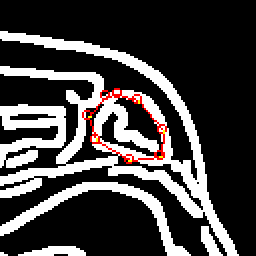
\includegraphics[scale=0.6]{images/ownimpl_result.png}
    \caption{Resultat der Erkennung der gewünschten Region anhand der eigenen Implementation in MATLAB\protect\footnotemark[1]{}}
\label{fig:ownimpl_result}
\end{figure}

\chapter{Fazit}
\label{chap:conclusion}

Die definierten Ziele konnten erreicht werden: Regionen werden generell in Bildern mittels aktiver Konturen als zusammenhängend erkannt.

Während mit der MATLAB-internen Method mehrere Regionen eines Bildes extrahiert werden können (siehe~\footnote{\url{http://www.mathworks.com/help/images/ref/activecontour.html\#btuvwkc}}), ist dies mit der selbst implementierten Variante zum jetzigen Zeitpunkt nicht möglich.

Ein interessanter Aspekt bei der Erkennung ist die Geschwindigkeit. Die MATLAB-interne Methode benötigt im Schnitt etwa 4.3 Sekunden zur Erkennung bei 300 Durchläufen. Die selbst Implementierte Variante benötigt hingegen im Schnitt etwa 3.5 Sekunden zur Erkennung bei 1000 Durchläufen.

\citeauthor*{Chan:2001:ACW:2318993.2320071} liefern mit ihrer Arbeit zur Erkennung von aktiven Konturen ohne erforderliche Kantenerkennung einen viel versprechenden Ansatz, siehe~\cite{Chan:2001:ACW:2318993.2320071}. MATLAB unterstützt diese Methode bereits. Bei einer einfachen Prüfung fiel dem Autor auf, dass die Erkennung der Fraktur mit dieser Methode nur unzuverlässig funktioniert (möglicherweise als Folge von unvollständiger Parametereingabe).

%---------------------------------------------------------------------------

% Glossary
%---------------------------------------------------------------------------
\cleardoublepage{}
\phantomsection{}
\addcontentsline{toc}{chapter}{Glossar}
\renewcommand{\glossaryname}{Glossar}
\printglossary{}
%---------------------------------------------------------------------------

% Bibliography
%---------------------------------------------------------------------------
\phantomsection{}
\addcontentsline{toc}{chapter}{Literaturverzeichnis}
\bibliographystyle{unsrtnat}
\bibliography{db/bibliography}{}
%---------------------------------------------------------------------------

% Listings
%---------------------------------------------------------------------------

\phantomsection{}
\addcontentsline{toc}{chapter}{Abbildungsverzeichnis}
\listoffigures

%\phantomsection{}
%\addcontentsline{toc}{chapter}{Tabellenverzeichnis}
%\listoftables
%---------------------------------------------------------------------------

% Index
%---------------------------------------------------------------------------

%\phantomsection{}
%\addcontentsline{toc}{chapter}{Stichwortverzeichnis}
%\renewcommand{\indexname}{Stichwortverzeichnis}
%\printindex
%---------------------------------------------------------------------------

% Attachment:
%---------------------------------------------------------------------------
\appendix
\settocdepth{section}
\begin{titlepage}


    \clearpage
    \vspace*{\fill}
    \begin{center}
        \begin{minipage}{.6\textwidth}
            \fontsize{26pt}{28pt}\selectfont
            Anhang
        \end{minipage}
    \end{center}
    \vfill % equivalent to \vspace{\fill}
    \clearpage


\end{titlepage}

\newpage 

% In den Anhang fügen Sie ein:
%  * Details des Projektpans, falls vorhanden
%  * Resultate und Zwischenresultate in Funktion der Projektiterationen
%  * Pflichtenheft / Anforderungsspezifikation (Stand Ende dritter Woche)
%  * Angaben zum Projektrepository
%  * Sitzungsprotokolle, falls vorhanden
%  * Weiterführende Erläuterungen zu den verwendeten Technologien, falls nötig
%  * Benutzerhandbuch, falls vorhanden und sinnvoll, es hier aufzulisten
%  * Installations- und Betriebsdokument, falls vorhanden und sinnvoll, es hier aufzulisten
% Unterlassen Sie das Anfügen von Listings.

\appendix

\section*{main.m}
\label{sec:appendix:main}
\lstinputlisting[language=Matlab,style=Matlab-editor]{appendix/main.m}

\newpage

\section*{Snake.m}
\label{sec:appendix:snake}
\lstinputlisting[language=Matlab,style=Matlab-editor]{appendix/Snake.m}

\newpage

\section*{SnakePoint.m}
\label{sec:appendix:snakepoint}
\lstinputlisting[language=Matlab,style=Matlab-editor]{appendix/SnakePoint.m}

\newpage

\section*{WindowUpdater.m}
\label{sec:appendix:windowupdater}
\lstinputlisting[language=Matlab,style=Matlab-editor]{appendix/WindowUpdater.m}

\newpage

\section*{test.m}
\label{sec:appendix:test}
\lstinputlisting[language=Matlab,style=Matlab-editor]{appendix/test.m}

%---------------------------------------------------------------------------

%---------------------------------------------------------------------------
\end{document} % chktex 17
